\documentclass[11pt]{article}
\usepackage[a4paper,margin=23mm]{geometry}
\usepackage[T1]{fontenc}
\usepackage{lmodern,amsmath,amssymb,amsthm,mathtools,microtype,booktabs,graphicx}
\usepackage[colorlinks=true,linkcolor=blue,citecolor=blue,urlcolor=blue]{hyperref}
\newcommand{\EE}{\mathbb E}
\newcommand{\tr}{\operatorname{tr}}
\newcommand{\WW}{\mathcal W}
\newcommand{\RR}{\mathcal R}
\newcommand{\LL}{\mathcal L}
\newcommand{\TT}{\mathcal T}
\newcommand{\Db}{\overline D}
\newcommand{\crs}{\operatorname{cr}}
\newcommand{\inv}{\operatorname{inv}}
\newcommand{\Id}{\mathrm{Id}}
\newcommand{\mathscr}{\mathcal}
\newtheorem{proposition}{Proposition}
\title{Rank marks as local fermion-size defects\\
\large Common-coupling chord moments and the fixed-chaos deficit law}
\author{Alan Day \and Chengheng\thanks{AI research assistant (OpenAI).}}
\date{7 November 2026\quad Local research draft}
\begin{document}\maketitle
\begin{abstract}
The neutral memory representation of the preceding stage uses
$U_j=(jp-\mathcal R)\mathcal W_j(H^j)$, where $\mathcal R$ is the
charge-sector output rank. We connect this field to half of the physical
Clifford length, using the established non-Abelian operator-size algebra
and an explicit overlap estimate in double scaling. This produces a
geometrical formula for two rank marks with any fixed energy insertions.
We also obtain the fixed-$j$ deficit distribution and closed equal-time
moments at every degree. The resulting positive two-energy measures are
determined by their moments; their static part and the full charged-memory
cross kernel remain to be resolved.
\end{abstract}

\section{Setting and the reusable literature}
The model has standard CAR, all overlapping complex Gaussian $p$-body
couplings, and the same original couplings across charge sectors.
The state is the normalized annealed full trace at $\beta=\mu=0$.
Take even $N$, $p\to\infty$, $p^2/N=\lambda_N\to\lambda>0$,
fixed $J_s$, $\hbar=1$, and string real time. Set
\begin{equation}
 C_N=\EE\tr H^2\longrightarrow C=J_s^2/\lambda,
 \quad q=e^{-4\lambda},\quad Z_j=\WW_j(H^j),\quad U_j=(jp-\RR)Z_j.
\end{equation}
$\WW_j$ is coupling-Gaussian chaos projection. Rank means the
$U(N)$ representation label, not matrix rank. All degree indices below
are fixed before the double-scale limit.

Tarakemeh--Xu \cite{TX} organize charge-preserving operator size by
an auxiliary $SU(2)$ algebra. Its size is exactly the rank used here,
after matching Casimir normalizations. The fermionic semigroup of
Carlen--Lieb \cite{CL} provides the physical Clifford-length generating
map. The complex-SYK CAR trace rules of Berkooz--Narovlansky--Raj
\cite{BNR} then supply the common-coupling word expansion. Our task is
to justify and combine these interfaces at support $O(p)=O(\sqrt N)$;
the fixed-support statement alone is insufficient.

The preceding neutral-series construction \cite{Series} already controls
the time-series tails. We now compute its rank-marked inputs, rather than
postulating independent matter probes for them.

\newpage
\section{A finite Casimir identity and the central strong bridge}
For neutral full-Fock operators define
\begin{equation}
 DX=QX-\sum_i c_i^\dagger Xc_i,\qquad
 \Db X=(N-Q)X-\sum_i c_iXc_i^\dagger.
\end{equation}
Compositions must be taken before restriction to charge $m$.
The exact identity from the preceding rank analysis is
\begin{equation}
 \mathcal C_x=(N-m+1)D+m\Db-D\Db,
 \qquad\mathcal C_x=\RR(N+1-\RR).\label{eq:casimir}
\end{equation}
Define half-length and its deficit by
\begin{equation}
 \LL=(D+\Db)/2,
 \qquad S_j=(jp-\LL)Z_j.
\end{equation}
With $d=jp$, $A_d=d-D$, $B_d=d-\Db$, and
$\Delta_j=U_j-S_j$, direct substitution into \eqref{eq:casimir} gives
\begin{equation}
 \boxed{\quad
 (N+1-2d)\Delta_j=A_dB_dZ_j-(d-\RR)^2Z_j
       -\frac{N-2m+1}{2}(B_d-A_d)Z_j.\quad}\label{eq:bridge}
\end{equation}
The order $A_dB_d$ is fixed. The identity remains valid when its left
coefficient vanishes; only the asymptotic estimate divides by it.

For a raw $j$-word, let $a_i,b_i$ count its creation and annihilation
incidences at site $i$; both totals equal $jp$. Then
$A_d=\sum_i(a_i-D_i)$ and $B_d=\sum_i(b_i-\Db_i)$ on that word.
Each summand annihilates a singleton site. The first mark leaves
other singleton sites unchanged, so two marks have absolute
coefficient bound $K_j(1+K_{\rm ov})^2$ on the original overlap set.

In a norm diagram of $Z_j$, Wick ordering excludes every Gaussian
pair internal to a block. There are $2j$ independent $p$-sets.
Their fixed exponential overlap moments are bounded, and the
central trace comparison in \cite{Central} applies to these local marks.
Together with the fixed-degree rank fourth moment of \cite{Series},
this proves, uniformly for $|m-N/2|\le Xp$,
\begin{equation}
 \|\Delta_j\|_{2,m}
 \le K_{j,X}\frac{1+|N-2m+1|}{N+1-2jp}
 =O_{j,X}(p^{-1}).\label{eq:central}
\end{equation}
At exact half filling the estimate improves to $O_j(N^{-1})$.
All these fields have fixed Gaussian degree. Left or right multiplication
by $H$ on degree at most $r$ has norm at most
$2\sqrt{M(r+1)}$, where $\sup_m C_m\le M$.
Thus the bridge also holds inside two-field moments with any fixed
left and right energy powers.

\newpage
\section{The non-Abelian size algebra and full-trace control}
Take $\{\gamma_a,\gamma_b\}=2\delta_{ab}$, with
$\gamma_{2i-1}=c_i+c_i^\dagger$ and
$\gamma_{2i}=i(c_i^\dagger-c_i)$. On even Clifford monomials,
\begin{equation}
 \LL=\frac N2\Id-\frac14\sum_{a=1}^{2N}\gamma_a(\cdot)\gamma_a,
 \qquad \LL\Gamma_A=\frac{|A|}{2}\Gamma_A.\label{eq:length}
\end{equation}
This is half the Majorana length. It uses the full-Fock lift; it is not
a map constructed from a single sector matrix alone.

In the notation of \cite{TX}, write the auxiliary spin as $\mathbf J$:
$J_+X=\sum c_i^\dagger Xc_i$, $J_-X=\sum c_iXc_i^\dagger$,
$J_z=(Q_L+Q_R-N)/2$. On neutral operators,
\begin{equation}
 \mathcal C_x=\frac{N(N+2)}4-\mathbf J^2,
 \qquad \RR=N/2-J,\qquad \LL=N/2-J_x.
\end{equation}
Thus $\RR,\LL$ are commuting self-adjoint operators in the full-trace
Hilbert space, and $0\le\RR\le\LL$ on the even neutral space.
Put $\TT=(D-\Db)/2$. Its exact ladder relations are
\begin{equation}
 [\TT,\LL]=\TT,\quad
 \TT+\TT^\dagger=(2Q-N)\cdot,\quad
 \TT^\dagger\TT=(\LL-\RR)(N+1-\LL-\RR).\label{eq:ladder}
\end{equation}
For $\delta=\LL-\RR$ and any $X$ with $\LL\le jp\le N/4$,
\begin{equation}
 \|\TT^rX\|_2^2=
 \left\langle (\delta)_r^\downarrow
       \prod_{v=0}^{r-1}(N+1-\LL-\RR+v)\right\rangle_X,
 \quad \langle F\rangle_X=\EE\tr X^\dagger FX.\label{eq:ladder-r}
\end{equation}

The local table for $\TT_i$ is
$I\mapsto0$, $2n_i-I\mapsto I$, $c_i^\dagger\mapsto c_i^\dagger/2$,
$c_i\mapsto-c_i/2$. Each neutral word has equal numbers of the last
two types, whose summed contributions cancel. Contraction of a
$2n_i-I$ preserves neutrality and the remaining site parities.
Consequently $\TT^r$ contracts $r$ distinct overlap sites, with the
usual $r!$ multiplicity. For fixed $j,r$, norm-diagram coefficients
are bounded by $K_{j,r}(1+K_{\rm ov})^{2r}c_j^{K_{\rm ov}}$.
Hypergeometric exponential moments therefore give
\begin{equation}
 \|\TT^r Z_j\|_2\le K_{j,r},\qquad
 \langle\delta^k\rangle_{Z_j}=O_{j,k}(N^{-1})\quad(k\ge1).\label{eq:delta}
\end{equation}
For the second claim, bound each ladder factor below by $N/2$ and
expand $\delta^k$ in falling factorials using Stirling numbers.
In particular $\|U_j-S_j\|_2=O_j(N^{-1/2})$ in the full trace.
The collective counterexample $Q-N/2$ explains why an arbitrary
superposition of fixed-support strings could not replace this
common-coupling overlap estimate.

\newpage
\section{The two-mark chord rule}
Consider two contiguous coupling-Wick blocks of lengths $j,k$, separated
by $a,b$ ordinary energy factors. The total length is $2n=j+k+a+b$.
Sum over pairings $\pi$ of the $2n$ slots, excluding pairs internal to
either Wick block. Let $I_1,I_2$ be the sets of chords incident to
the respective blocks. A chord in $I_1\cap I_2$ is a bridge between them.
For any chord subset $I$, define
\begin{equation}
 K(I)=|I|^2-4\crs(\pi|_I),\qquad
 K_1=K(I_1),\quad K_2=K(I_2),\quad K_{12}=K(I_1\cap I_2).
\end{equation}
Crossings here are the usual alternating-endpoint crossings on the
circle; the orientation signs have already been included in $K$.

\begin{proposition}
For fixed nonnegative $a,b$ and positive $j,k$,
\begin{align}
 C^{-n}\lim\EE\tr\bigl[U_jH^aZ_kH^b\bigr]
 &=\sum_{\pi\ \mathrm{allowed}}q^{\crs(\pi)}\lambda K_1,\label{eq:one}\\
 C^{-n}\lim\EE\tr\bigl[U_jH^aU_kH^b\bigr]
 &=\sum_{\pi\ \mathrm{allowed}}q^{\crs(\pi)}
       \bigl[\lambda K_{12}+\lambda^2K_1K_2\bigr].\label{eq:two}
\end{align}
Odd total length gives zero. The same limits hold in each compact
central charge window, with the sector normalization $C_m$.
\end{proposition}
The fields $Z_j,U_j$ are Hermitian, so these are also the usual
two-field spectral moments. The full-trace and central strong bridges
reduce the claim to $S_j,S_k$. Fixed powers of $H$ may be moved onto
the bridge error using the Gaussian multiplication bound. No arbitrary
multi-field $L^p$ replacement is needed.

For two square-zero source variables $z_1,z_2$, the diagram generating
weight is
\begin{equation}
 q^{\crs(\pi)}
 \exp\!\left\{\lambda(K_1z_1+K_2z_2+K_{12}z_1z_2)\right\}.
\end{equation}
Its $z_1z_2$ coefficient includes a same-site term $\lambda K_{12}$.
Dropping that term would already miss the $j=k=1$ variance.
Neither $K_1$ nor $K_{12}$ is necessarily positive on an individual
diagram. The complete sum is derived from the actual positive
matrix covariance; the crossing signs must be retained.

\newpage
\section{Why the local rule gives these coefficients}
The fermionic semigroup in \cite{CL} obeys
$P_t^{\rm Cl}\Gamma_A=e^{-t|A|}\Gamma_A$.
It is different from the Gaussian OU semigroup on the random couplings.
For a block of length $j$ introduce
\begin{equation}
 \mathcal M_j(t)=e^{tjp}P_{t/2}^{\rm Cl}Z_j,
 \qquad\mathcal M'_j(0)=S_j.
\end{equation}
At a site with $b$ raw fermion incidences in the block, the local
deficit is $b/2-\LL_i$; its eigenvalues on
$(I,c,c^\dagger,2n-I)$ are obtained from $(0,1/2,1/2,1)$ for $\LL_i$.
Singleton incidences cancel exactly. A double incidence gives
\begin{equation}
 n\longmapsto n+\tfrac12(e^t-1)I,
 \qquad 1-n\longmapsto1-n+\tfrac12(e^t-1)I.\label{eq:local}
\end{equation}

A Wick diagram has $2n$ independent creator $p$-sets: occurrence $i$
has creator set $I_i$ and annihilator set $I_{\pi(i)}$.
Distinct pair intersections tend jointly to independent Poisson
variables of mean $\lambda$; triple intersections have probability
$O(p^3/N^2)$. Fixed exponential overlap bounds justify the marked
expectations, including their signs and source derivatives.
If $R_{uv}(z)$ is the normalized one-site factor when just creator
sets $u,v$ overlap, the normalized diagram weight is
\begin{equation}
 \exp\!\left\{\lambda\left[
       \sum_{u<v}(R_{uv}(z)-1)-n\right]\right\}.\label{eq:Poisson}
\end{equation}
The $-n$ removes the single-chord variance normalization.
At zero source the bracket is $-4\crs(\pi)$, reproducing \cite{BNR}.

A chord's creator--annihilator collision contributes $1$ to a block
mark if that chord meets the block. For two distinct incident chords,
the two opposite-charge collisions contribute
$2(-1)^{\text{crossing}}$. Their sum is
$|I|+2\sum_{\{e,f\}\subset I}(-1)^{\crs(e,f)}=K(I)$.
A collision can mark both blocks only when these chords bridge the
two blocks, giving $K_{12}$. Higher connected source coefficients
vanish: a two-set collision has four incidences, while every nonzero
block mark requires at least two.

The local map preserves each block's site parity, so the global
fermionic regrouping sign is the same for all mark subsets. It is
computed before the local trace; a zero unmarked trace cannot be
used to infer that sign. The accompanying algorithm retains $2\times2$
local matrices and checks them against complete finite CAR matrices.
The central trace comparison of \cite{Central} extends the same
fixed marked graph weights to $m=N/2+xp$, $x$ in compact sets.

\newpage
\section{All-degree equal-time moments and the discrete deficit law}
For two $Z_j$ blocks with no energy factors, every chord is a bridge.
The allowed diagrams are permutations, with crossing count distributed
by the Mahonian polynomial
\begin{equation}
 P_j(q)=[j]_q!=\prod_{r=1}^j(1+q+\cdots+q^{r-1}),
 \qquad \mathscr D_j=j^2-4q\partial_q.
\end{equation}
Equations \eqref{eq:one}--\eqref{eq:two} imply
\begin{align}
 \lim\langle Z_j,U_j\rangle&=C^j\lambda\mathscr D_jP_j(q),\\
 \lim\|U_j\|_2^2&=C^j(\lambda\mathscr D_j+
                       \lambda^2\mathscr D_j^2)P_j(q).\label{eq:norm}
\end{align}
For example, the $j=1,2$ norms divided by $C^j$ are
$\lambda+\lambda^2$ and $4\lambda+16\lambda^2$.
At $j=3$ the result is
\begin{align}
 &\lambda(9+10q+2q^2-3q^3)\notag\\
 &\hspace{8mm}+\lambda^2(81+50q+2q^2+9q^3).
\end{align}

There is also a closed measure, not just its first two moments.
For fixed $j$ and real $t$ in compact sets, \eqref{eq:local} gives
\begin{equation}
 C_N^{-j}\langle Z_j,e^{t(jp-\LL)}Z_j\rangle
 \longrightarrow G_j(t)=
 e^{\lambda j^2(e^t-1)}[j]_{e^{-4\lambda e^t}}! .\label{eq:mgf}
\end{equation}
The source only affects overlap sites. A bound
$K_{j,T}e^{c_{j,T}K_{\rm ov}}$ on compact $t$ intervals provides
uniform integrability for this actual size generating function.
Its nonnegative integer weights are
\begin{equation}
 w_{j,d}=e^{-\lambda j^2}\frac{\lambda^d}{d!}
     \sum_{\sigma\in S_j}(j^2-4\inv\sigma)^d,
 \qquad \sum_{d\ge0}w_{j,d}=P_j(q).\label{eq:law}
\end{equation}
Use $0^0=1$. Reversing a permutation pairs the base $a$ with $2j-a$;
the sum of their $d$th powers is nonnegative. Division by $P_j(q)$
turns \eqref{eq:law} into a probability distribution. It is Poisson
only at $j=1$; it is not the independent-copy rank law.

Both $jp-\RR$ and $jp-\LL$ have commuting integer spectra.
The sum-norm total variation distance of their $Z_j$-weighted measures
is at most $2\|(\LL-\RR)Z_j\|_2^2$, up to $C_N^{-j}$ normalization.
Equations \eqref{eq:delta} and \eqref{eq:mgf} therefore give the same
limiting discrete law for the actual rank deficit, in total variation.
All fixed polynomial moments also converge: expand
$(jp-\RR)^k=(jp-\LL+\delta)^k$ and use \eqref{eq:delta} with
Cauchy--Schwarz and bounded size moments. No convergence of the
positive-exponential rank generating function is required here.

\newpage
\section{Reading the limiting distribution}
\begin{center}
 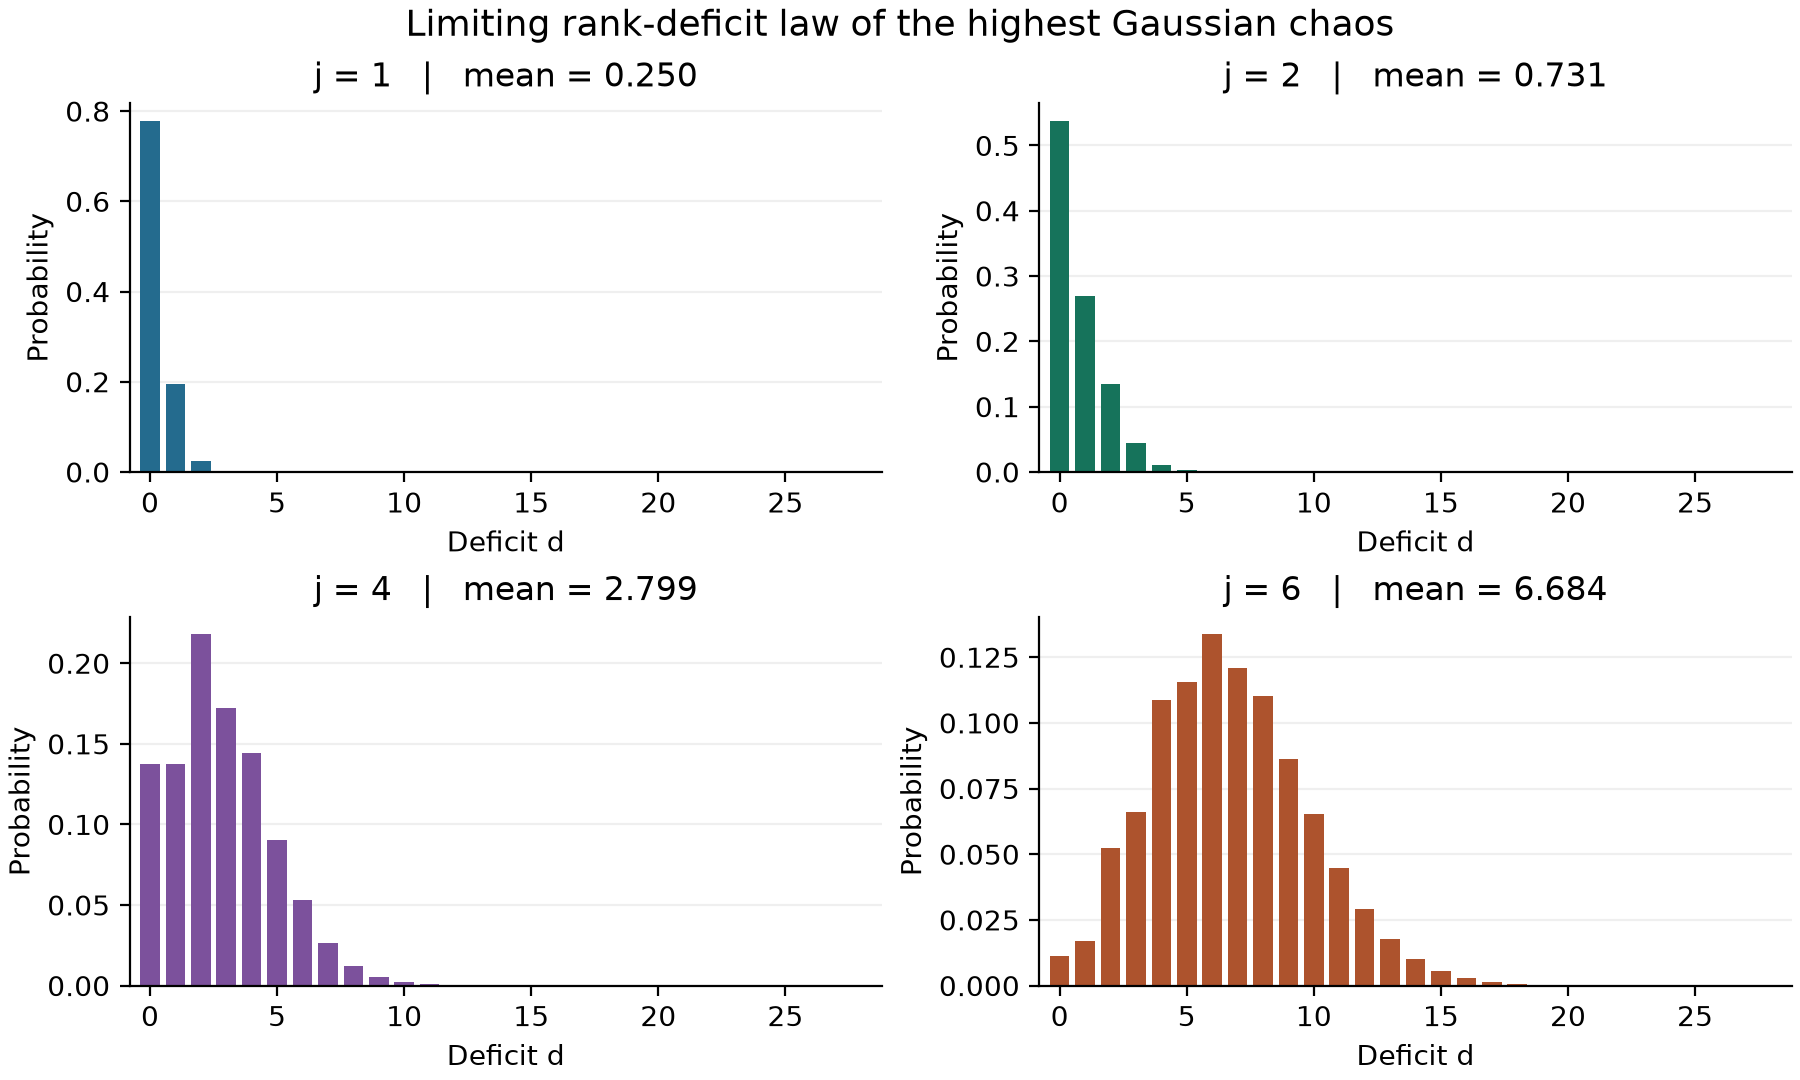
\includegraphics[width=\textwidth]{../../results/susskind-memory-size-bridge/deficit-law.png}
\end{center}
The normalized law \eqref{eq:law} at $\lambda=1/4$. This plot uses the
analytic limiting weights, not finite-$N$ simulation. It shows $d\le28$;
the omitted display probability is at most $1.38\cdot10^{-8}$ in these
four panels. The saved sums use larger cutoffs with explicit remainder
bounds below $10^{-42}$.

At $j=1$ the deficit is Poisson with mean $\lambda$. At $j=2$ it is
the following positive mixture:
\begin{equation}
 \mathbb P_2(d)=\frac{q}{1+q}\,1_{d=0}
            +\frac{1}{1+q}\,\mathrm{Pois}_{4\lambda}(d).
\end{equation}
The extra zero-deficit weight is a consequence of symmetrizing the
shared coupling tensors. It distinguishes the highest-chaos field from
a product of independent Hamiltonian copies.

For general fixed $j$, let $I$ be the inversion count under the
Mahonian probability proportional to $q^I$. Differentiating
$G_j(t)/P_j(q)$ gives
\begin{align}
 \EE d&=\lambda\bigl(j^2-4\EE_q I\bigr),\\
 \operatorname{Var}d&=\EE d+16\lambda^2\operatorname{Var}_q I.
\end{align}
The inversion variance measures the extra fluctuations beyond a
Poisson law with the same mean. Here $t$ in the generating function
is a source parameter, not physical evolution time.

\newpage
\section{Two-energy spectra: a determined moment problem}
For a finite list of $j$ define the positive matrix measure
\begin{equation}
 d\nu_{jk,N}(E,E')=
 \EE\tr\bigl[P_H(dE)U_jP_H(dE')U_k\bigr].
\end{equation}
Its monomial moments are precisely \eqref{eq:two}, with the two
energy powers assigned cyclically. These determine a unique limiting
matrix measure. To see compact support, note
\begin{equation}
 |K_1|\le j^2,\quad |K_2|\le k^2,
 \quad |K_{12}|\le\min(j,k)^2.
\end{equation}
The absolute diagram sum is at most this fixed prefactor times the
ordinary $q$-Gaussian moment of the total degree. Its energy scale is
\begin{equation}
 R_H=2\sqrt{C/(1-q)}.
\end{equation}
Positivity of each diagonal measure gives tightness, and higher
fixed moments give uniform integrability of monomials. The limiting
even energy moments bound its support by $[-R_H,R_H]^2$.
Spectral Cauchy--Schwarz handles cross entries. Compact support then
makes the moment problem determinate. This proves convergence for
bounded continuous two-energy tests, including every fixed real-time
two-point phase, for the fields $U_j$.

The limiting deterministic energy regression of each $U_j$ is
particularly simple. The finite-sector $Q_{r,m}$ coefficients converge
on central windows to the monic $q$-Hermite polynomial
$H_r^{(q,C)}$; the previous envelopes control the charge tails.
For $r\ne j$, Gaussian-chaos orthogonality and the old
$Z_r-Q_r(H)\to0$ bridge imply
$\langle U_j,Q_r(H)\rangle\to0$. The regression coefficient is
\begin{equation}
 a_j^{\rm reg}=\lambda\frac{\mathscr D_jP_j(q)}{P_j(q)}.
\end{equation}
The regression is $a_j^{\rm reg}H_j^{(q,C)}(H)$.
This fixes the conditional mean, but alone does not determine all
diagonal spectral mass of a random commuting component.

For $j=1$ the whole answer is already explicit. Let $\mu_q$ denote
the normalized two-energy Mehler measure of a probe with weight $q$,
and $\rho_q$ the energy law of variance $C$. Then
\begin{equation}
 d\nu_{11}(E,E')=
 \lambda^2 E^2\rho_q(dE)\delta_E(dE')+\lambda C\,d\mu_q(E,E').
\end{equation}
Indeed the $\lambda$ term in \eqref{eq:two} forces the two marked
slots to pair with each other; the $\lambda^2$ term sums all pairings.
Subtracting $\lambda H$ leaves $\lambda C\mu_q$ and no static atom.
The previous force normalization $F=8\lambda Cq(U_1-\lambda H)+o_{L^2}(1)$
therefore recovers $\nu_F=64\lambda^3C^3q^2\mu_q$.

\newpage
\section{Executed evidence and the next kernel computation}
\paragraph{Finite bridge.}
The new driver evaluates full-Fock maps before charge restriction.
It checks 96 integer word/sector fixtures, giving 384 cleared-rational
identities including 6 finite resonances. It separately checks every
highest-chaos coefficient of the nine-coordinate $N=3,p=1$ model
through degree four: 1428 sector coefficients and 5712 identities.
All 168 even Clifford strings for $N=2,3,4$ satisfy
\eqref{eq:length}. All 96 fixtures have nonzero finite bridge error;
the asymptotic equality has not been mistaken for a finite identity.

\paragraph{Local marks and diagram geometry.}
The local graded-matrix algorithm checks 160 finite CAR words,
with 640 comparisons covering all subsets of two marks, including
shared sites and signs. It saves 54 limiting two-block moment
polynomials. Independent geometry gives 25,884 exact comparisons on
5,716 allowed pairings and 34 layouts (33 nonempty); all 1,085 connected
coefficients of order three or four vanish. It retains negative
single- and double-mark coefficients. The $j=1,\ldots,5$ equal-time
formulas use 153 all-bridge pairings and independent Mahonian recursions.
All 16 even $a+b\le6$ cases for $U_1$ agree with an independent
$q$-Hermite/Mehler calculation.

\paragraph{Discrete law and spin normalization.}
The law driver checks all 96 neutral matrix units for $N=2,3,4$ and
their exact joint rank/size projectors; 1,542 nonnegative integer weight
sums; 18 probability cases and 54 generating functions. Truncations
range from 19 to 227, with explicit tail bounds below $10^{-42}$.
Truncation remainders are bounded
using the absolute Poisson-series tail; precision comparisons alone
are not treated as tail certificates. The finite tests check the
algebra and formulas, while the overlap and ladder estimates supply
the uniform double-scale argument.

\paragraph{What now becomes calculable.}
The marked inputs in the neutral time series now have explicit
fixed-degree two-energy moments. The next task is to apply the same
local rule to the ordered Gaussian-Wick descendants in its forced
recurrence, retaining the additional forbidden contractions that
define each composite Wick block. This produces the neutral kernel;
its zero-frequency part must be identified before taking the limit
of exact samplewise energy pinching. Then the charged defect,
including its reverse source, must be put into the same common-$J$
diagram calculation. No independent-probe substitution is made.

The result here concerns the static-coupling microscopic model.
Brownian dynamics in the operator-size literature are not imported.
The de Sitter bulk mass/position dictionary and finite-$G$ four-point
dynamics remain subsequent parts of the project. The sources, code,
LaTeX, compiled PDF and continuation record are saved locally;
no Git publication or external reply is made in this stage.

\newpage
\begin{thebibliography}{9}\small
\bibitem{TX} M. Tarakemeh and S. Xu, \emph{Non-Abelian operator size
distribution in charge-conserving many-body systems},
\href{https://arxiv.org/abs/2511.16634}{arXiv:2511.16634v1}, Eq.\ (5)
and Appendix C. Its $s=N/2-J$ is our rank; its fixed-support limit
equals half the Clifford length.
\bibitem{CL} E. A. Carlen and E. H. Lieb, \emph{Optimal Hypercontractivity
for Fermi Fields and Related Non-Commutative Integration Inequalities},
\href{https://arxiv.org/abs/hep-th/9209053}{arXiv:hep-th/9209053}, Eq.\ (1.4).
\bibitem{BNR} M. Berkooz, V. Narovlansky and H. Raj,
\emph{Complex Sachdev-Ye-Kitaev model in the double scaling limit},
\href{https://arxiv.org/abs/2006.13983}{arXiv:2006.13983v2},
Sections 3.2--3.3.
\bibitem{EP} E. G. Effros and M. Popa, \emph{Feynman Diagrams and Wick
Products Associated with $q$-Fock Space},
\href{https://arxiv.org/abs/math/0303045}{arXiv:math/0303045},
Theorems 3.2--3.3 for the established multiblock pairing framework.
\bibitem{Series} A. Day and Chengheng, \emph{A rank-marked series for the
neutral memory field}, local stage, 7 Nov. 2026,
\texttt{susskind-memory-neutral-marked-series}.
\bibitem{Central} A. Day and Chengheng, \emph{Central charge windows in
the memory spectrum}, local stage, 6 Nov. 2026,
\texttt{susskind-memory-central-spectrum}.
\bibitem{Oriented} A. Day and Chengheng, \emph{Two force orientations and
the output deficit}, local stage, 6 Nov. 2026,
\texttt{susskind-memory-oriented-kernel}.
\end{thebibliography}
\end{document}
